
\chapter{発行キュー(IQ:Issue Queue)}
\label{sec:basic_IQ}
本章では,本研究の研究対象である、IQ に関して説明する.まず,IQ の概要と動作を\refsec{iq_abst}で説明したあと,IQ の回路構成を\refsec{iq_circuit}で述べる.その後,\refsec{iq_scheme}でIQ の方式に関して説明する.

\section{概要と動作}
\label{sec:iq_abst}
IQ はアウト・オブ・オーダ実行を行うプロセッサにおいて,リネームされた命令を保持し,実行順序をスケジューリングして,機能ユニットへ発行する回路である.IQ は,ディスパッチ,発行,ウェイクアップと呼ばれる 3 種類の動作を行う.以下でそれぞれの動作に関して説明する.

\begin{itemize}
  \item ディスパッチ:リネームされた命令は,IQ にエントリが割り当てられ,命令の情報が格納される.この動作をディスパッチと呼ぶ.ディスパッチの動作は,IQ の方式により異なる.IQ の方式に関しては,\refsec{iq_scheme}で詳しく説明する.
  \item 発行:IQ 内の命令のうち,ソース・オペランドが両方共レディとなった命令は,依存関係が解消し,実行が可能となる.このような命令を実行ユニットに送出する動作を発行と呼ぶ.なお,発行可能な命令が機能ユニットの数を超える場合(このような場合を発行コンフリクトと呼ぶ)は,各命令の発行優先度に基づき命令を選択して発行する.発行された命令のエントリは IQ より削除される. 
  \item ウェイクアップ:命令が発行されると,その命令のディスティネーション・オペランドのタグと発行キュー内にある全命令のソース・オペランドのタグの比較が行われる.比較が一致した場合には,対応するソース・オペランドのレディ・ビットをセットする.この動作をウェイクアップと呼ぶ.両方のオペランドがレディとなった命令は,依存が解消したため発行可能となる.
\end{itemize}

\begin{figure}[thb]
  \centering
  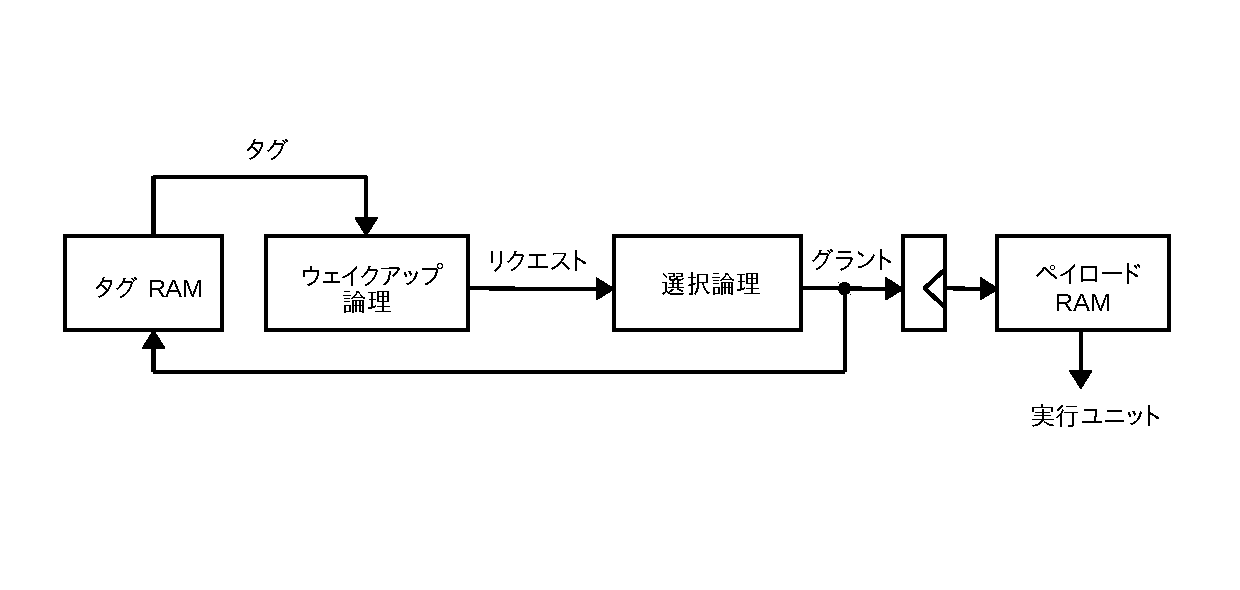
\includegraphics[keepaspectratio, scale=.8]{iq_logic}
  \caption{IQ の回路構成}
  \label{fig:iq_logic}
\end{figure}

\section{回路構成}
\label{sec:iq_circuit}
\fig{iq_logic}に IQ の回路構成を示す.IQ はウェイクアップ論理,選択論理,タグ RAM,ペイロード RAM と呼ばれる 4 つの回路より構成される.以下で各回路に関して説明する.また,IQ の回路のうちウェイクアップ論理は提案手法に関わる重要な回路であるため,\refsec{wakeup_logic}にて詳細に説明する.

\begin{itemize}
  \item ウェイクアップ論理:命令感の依存関係を管理し,他の命令との依存関係が解消された命令に対して発行要求(リクエスト信号)を出す.
  \item 選択論理:資源制約を考慮して,発行を要求された命令の中からそれを許可する命令を選択肢,発行許可信号(グラント信号)を出力する.この選択においては,回路構成の単純化のために IQ の先頭のエントリの命令をより優先する.
  \item タグ RAM:発行待機中の命令のディスティネーション・タグを保持する回路で,選択論理から発行許可信号が送られると,対応する命令のタグを読み出し,それをウェイクアップ論理へ送る.
  \item ペイロード RAM:発行待機中の命令の命令のコードを保持する.選択論理から発行許可信号が送られると,対応する命令のコードを実行ユニットに送出する. 
\end{itemize}

\begin{figure}[thb]
  \centering
  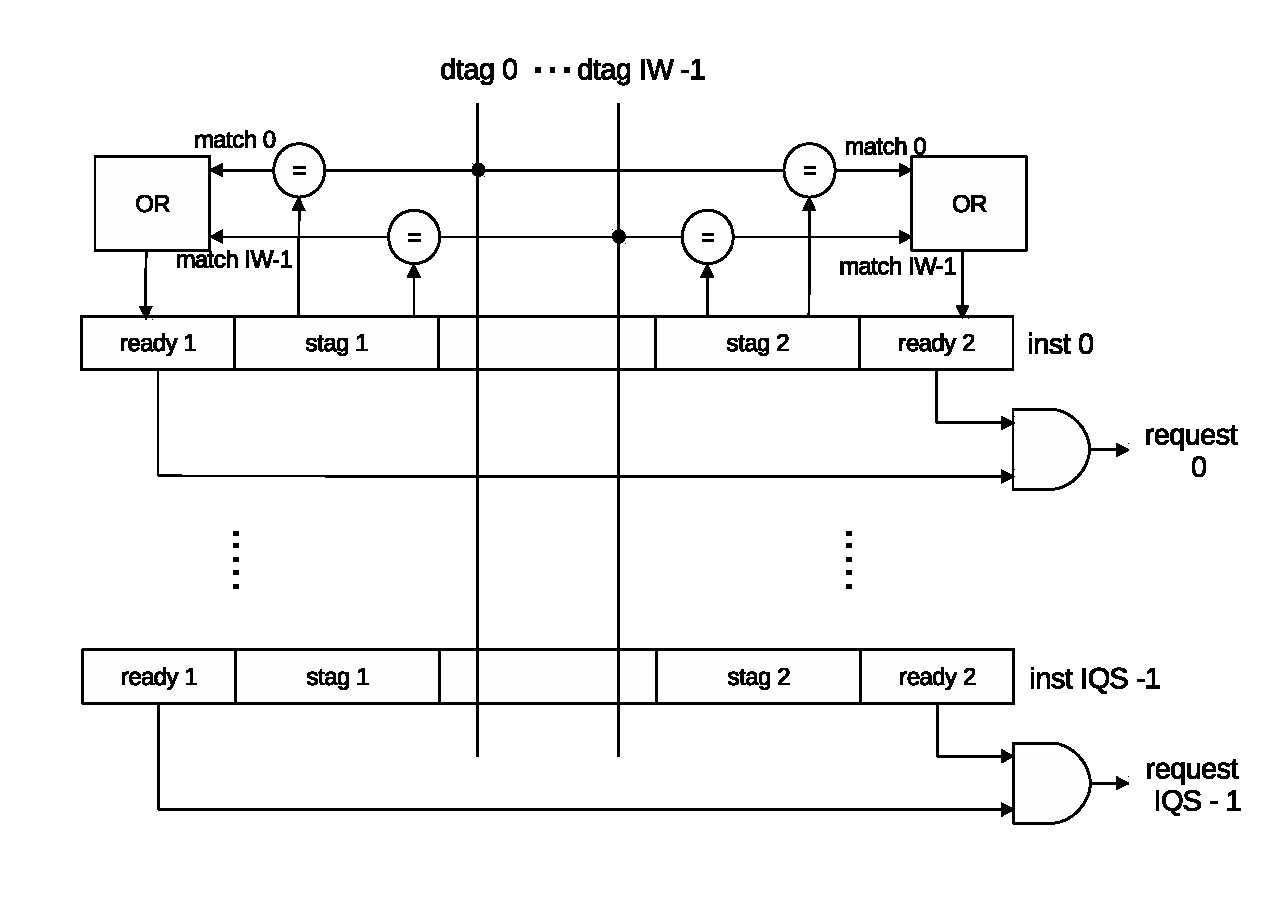
\includegraphics[keepaspectratio, scale=.8]{wakeup_logic}
  \caption{ウェイクアップ論理}
  \label{fig:wakeup_logic}
\end{figure}

\begin{figure}[htb]
  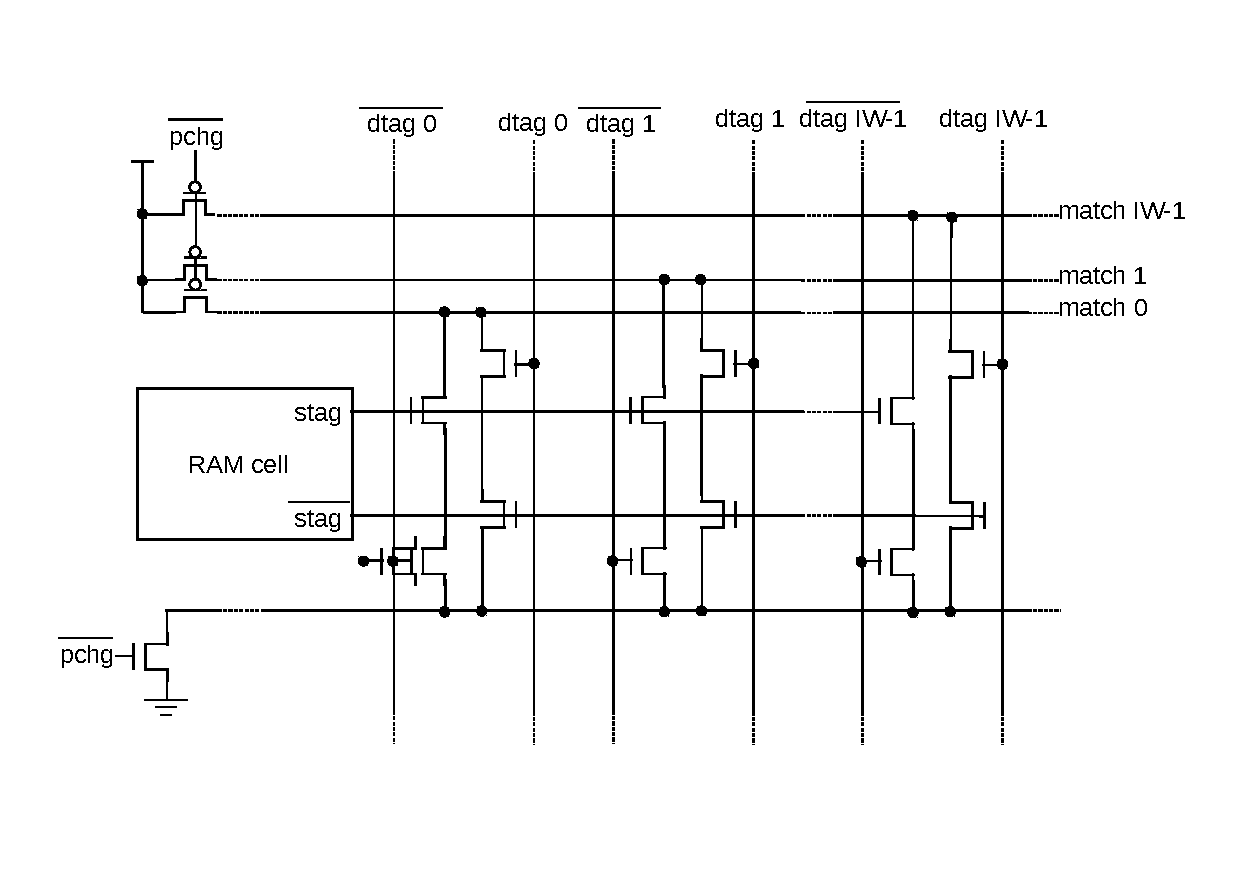
\includegraphics[keepaspectratio, scale=.8]{cam}
  \caption{タグ比較器の CAM 回路}
  \label{fig:cam}
\end{figure}

\subsection{ウェイクアップ論理}
\label{sec:wakeup_logic}
\fig{wakeup_logic}に,ウェイクアップの回路を示す.図中の $IW$ は発行幅を,$IQS$ は発行キューのエントリ数を表す.ウェイクアップでは,$IW$ 個のディスティネーション・タグ(dtag)が発行キュー内の全命令に放送される.各命令は 2 つのソース・タグ(stag)を保持しており,放送されたディスティネーション・タグと比較が行われる.いずれかのディスティネーション・タグとソース・タグが一致した場合,そのソース・オペランドのレディ・ビットがセットされる.2 つのレディ・ビットがセットされた命令は発行が可能となるため発行要求が出力される.

\fig{cam}に発行キューに使用されるタグ比較器の CAM 回路を示す.同図は,ソース・タグ 1 ビット分の比較回路を表す.同図に示すように,高速化のため通常ダイナミック論理によって構成される.比較の動作は,次のように行われる.まず,マッチ線がプリチャージされる.次にデスティネーション・タグが放送され,比較が行われる.タグが不一致であれば,直列に接続された 2 つのプルダウン・トランジスタが両方とも ON となり,マッチ線がディスチャージされる.タグが一致する場合,マッチ線は $H$ の状態が維持される.比較器はマッチ線のディスチャージ時に電力を消費する.

\section{IQ の方式}
\label{sec:iq_scheme}
これまで,IQ の方式としてシフト・キュー,サーキュラ・キュー,ランダム・キューの 3 つの方式が提案されている.各方式に関して説明したのち,現在主流な方式であるエイジ論理付きのランダム・キューに関して説明する.

\subsection{シフト・キュー}
シフト・キューは,最も古くに提案され,商用プロセッサに使用された IQ の方式である~\cite{Farrell1998}.シフト・キューでは,IQ の先頭のエントリより順に命令をディスパッチする.これにより,古い命令に高い発行優先度を与えることができる.\footnote{一般に,古い命令から優先的に発行すると,性能がより高くなることが知られている.}

また,シフト・キューでは命令を発行したエントリの空きを詰めるコンパクションを行うことにより,高い容量効率も達成することができる.正しい発行優先度と,高い容量効率を同時に達成するため,シフト・キューは IQ の方式の中で最も高い性能を得ることができる.

一方でシフト・キューには,コンパクションの回路が非常に複雑で,また消費電力が非常に大きいという欠点がある.そのため,シフト・キューはスケーリングが困難となっており,現在のプロセッサには使用されていない.

\subsection{サーキュラー・キュー}
サーキュラ・キューは,シフト・キューにおいて問題であったコンパクションを行わない方式である~\cite{Abella:survey2003}.IQ は,ヘッド・ポインタとテール・ポインタを用いてサーキュラー・バッファとして管理される.

サーキュラー・キューでは,既に空いているが,命令をディスパッチできないエントリが発生し,IQ の容量効率がシフト・キューと比較して低下してしまう.また,ヘッド・ポインタとテール・ポインタの位置が逆転するラップ・アラウンドが生じた際には,新しい命令に高い優先度が与えられる優先度逆転が起き,選択論理が正しい優先度で命令を選択できない.これらの理由から,サーキュラー・キューはシフト・キューと比較して性能が低下する.

特に,容量効率が低下する影響は大きく,現在のプロセッサには使用されていない.

\subsection{ランダム・キュー}
近年は,回路の単純化や電力削減のため空いているエントリに単純にディスパッチするランダム・キューが使用されている.ランダム・キューでは IQ の容量を無駄にすることがなく,高い容量効率を達成する.その一方で,命令が年齢とは無関係にランダムに並ぶため,正しい優先度で命令を発行することが出来ない.

ランダム・キューでは,発行キューの空きエントリのインデクスを保持するフリー・リストを用意する.ディスパッチ時には,フリー・リストから読み出したインデクスが指す発行キューのエントリに命令を書き込む.発行キューから命令が発行されエントリが無効化されると,そのインデクスをフリー・リストへ返す.フリー・リストは FIFO バッファで管理される.

\subsection{エイジ論理付きランダム・キュー}
ランダム・キューにおける発行優先度の欠点を緩和するため,ランダム.キューは一般にエイジ論理と併用される.エイジ論理は選択論理と並列に動作する回路で,発行要求が出された命令の中で最も古い 1 命令を選ぶ.最も古い命令はクリティカル・パス上の命令である可能性が高いため,これを優先して発行することができ,結果としてエイジ論理付きランダム・キューは通常のランダム・キュート比較して性能が大きく向上する.

本研究における IQ は,エイジ論理付きのランダム・キューを使用する.

\section{IQ の問題点}
\label{sec:iq_problem}
IQ は電力密度の大きいホットスポットとして知られている.この主な原因は,ウェイクアップ論理での消費電力である.論文によると,ウェイクアップ論理の消費電力はIQ 全体の20\% であり,削減の必要がある.

ウェイクアップ論理での消費電力が大きい理由として,タグ比較回路が挙げられる.タグ比較に使用する CAM は,$IQS \times IW \times 2$個必要である.ここで,IQS は IQ のエントリ数, IW は発行幅 を表す.現在想定しているプロセッサ構成では,IQS は 128 エントリ,IQ は 8 命令であるため,CAM の総数は 2048 個となる.

これだけ多くの CAM が毎サイクル動作するため,ウェイクアップ論理の電力密度は大きくなる.本研究では,ウェイクアップ時のタグ比較によって生じる消費電力を削減することを目的とする.












% 図を使う例: figure 環境を使用

% \begin{figure}[tb]
%   \centering
%   \includegraphics[scale=.5]{hoge.eps}
%   \caption{例1}
%   \label{fig:hoge}
% \end{figure}



% 副図を使う例: minipage と subcaption を使用

% \begin{figure}[tb]
%   \begin{minipage}[htb]{1\hsize}
%     \centering 
%     \includegraphics[keepaspectratio, scale=0.8]{hap_pipeline.eps}
%     \vspace{.3cm} % <-- vspace で縦方向の位置を調節できる
%     \subcaption{従来のパイプライン (HAP: Hit-Assuming Pipeline)}
%     \label{fig:hap_pipeline}
%   \end{minipage}
%   \begin{minipage}[htb]{.97\hsize}
%     \vspace{1.3cm}
%     \centering
%     \includegraphics[keepaspectratio, scale=0.8]{map_pipeline.eps}
%     \vspace{.3cm}
%     \subcaption{MAP: Miss-Assuming Pipeline}
%     \label{fig:map_pipeline}
%   \end{minipage}
%   \vspace{.8cm}
%   \caption{各パイプラインの命令処理工程}
%   \label{fig:pipeline}
% \end{figure}


